\documentclass[letterpaper, 10 pt, conference]{sty/ieeeconf}

\IEEEoverridecommandlockouts

\overrideIEEEmargins

\usepackage{graphics}
\usepackage{epsfig}
\usepackage{amsmath}
\usepackage{amssymb}
\usepackage{txfonts}
\usepackage{tikz}
\usepackage{sty/tkz-base}
\usepackage[T1]{fontenc}
\usepackage{cite}

\usetikzlibrary{shapes,decorations,shadows}
\usetikzlibrary{decorations.pathmorphing}
\usetikzlibrary{decorations.shapes}
\usetikzlibrary{fadings}
\usetikzlibrary{patterns}
\usetikzlibrary{calc}
\usetikzlibrary{decorations.text}
\usetikzlibrary{decorations.footprints}
\usetikzlibrary{decorations.fractals}
\usetikzlibrary{shapes.gates.logic.IEC}
\usetikzlibrary{shapes.gates.logic.US}
\usetikzlibrary{fit,chains}
\usetikzlibrary{positioning}
\usepgflibrary{shapes}
\usetikzlibrary{scopes}
\usetikzlibrary{arrows}
\usetikzlibrary{backgrounds}
\tikzset{latent/.style={circle,fill=white,draw=black,inner sep=1pt, 
minimum size=20pt, font=\fontsize{10}{10}\selectfont},
obs/.style={latent,fill=gray!25},
const/.style={rectangle, inner sep=0pt},
factor/.style={rectangle, fill=gray!25,minimum size=15pt, inner sep=1pt,draw=black},
>={triangle 45}}

\DeclareMathOperator*{\argmax}{arg\,max}
\DeclareMathOperator*{\argmin}{arg\,min}

\begin{document}

\title{\LARGE \bf
Self-supervised Calibration for Mobile Robot Sensors
}

\author{
\authorblockN{
J\'{e}r\^{o}me Maye,
Paul Furgale,
and Roland Siegwart}
\authorblockA{
Autonomous Systems Lab, ETH Zurich, Switzerland\\
email: \{jerome.maye, paul.furgale, roland.siegwart\}@mavt.ethz.ch}
}

\maketitle

\begin{abstract}
In this paper, we address the problem of sensors calibration for mobile robots.
In particular, we are aiming towards an automated system ready to be deployed
for long-term and online operation in the hands of non-experts. To this end, we
augment the classical SLAM formulation with calibration parameters and derive
an MAP estimator that is computed using a Gauss-Newton algorithm. Degenerate
dimensions in sensor data are identified by means of QR decomposition and
automatically discarded from the optimization via a truncated method, such that
only observable parts are exploited. Finally, incoming sensor data is processed
in batch and selected using an information theoretic measure. Through an
extensive set of simulated and real-world experiments, we demonstrate that our
method outperforms state-of-the-art algorithms in terms of applicability,
accuracy, and speed.

\end{abstract}

\section{Introduction\label{intro}}
Every robotic system has some set of parameters---scale factors, sensor
locations, link lengths, etc.---that are needed for state estimation, planning,
and control. Despite best efforts during construction, some parameters will
change over the lifetime of a robot due to normal wear and tear. In the best
case, incorrect parameter values degrade performance. In the worst case, they
cause critical safety issues.

We are interested in developing automated systems that are capable of robust
long-term deployment in the hands of non-experts, so the identification and
update of these parameter values is highly important.

As an example, consider a camera-based collision avoidance system intended for
deployment in a consumer automobile. For the vehicle to be able to avoid
collisions, the pose of each camera with respect to the vehicle coordinate
system must be known precisely so that obstacle positions can be transformed
from camera coordinates into vehicle coordinates. However, a consumer vehicle
will have no access to special calibration hardware or expert data analysis.
In such a scenario, the vehicle must be capable of self-supervised
recalibration. This problem is inherently difficult for a number of reasons that
we will briefly discuss here.

{\bf 1) Parameters change over time}---although the vehicle may be factory
calibrated, the transformations can change slowly over time due to vibration,
thermal expansion, loose parts, or any number of other common problems that
follow from normal usage.

{\bf 2) Parameters must be inferred from the data}---as the cameras may be
installed in different places on the vehicle, their pose cannot be measured
directly. Instead, the transformations must be inferred from the data produced
by the full system. However, this is only possible if the motion of the vehicle
renders the parameters {\em observable}\footnote{Informally, observability
means that the parameters can be inferred from some local batch of measurement
data~\cite{jazwinski70stochastic}}.

{\bf 3) Normal operation may result in unobservable directions in parameter
space}---unfortunately, for this and many other practical problems normal
operation may not render all directions in parameters space observable. In this
example, when two cameras do not share an overlapping field of view, planar
motion renders the calibration problem
degenerate\footnote{See~\cite{lebraly10calibration} for a handy table of
degenerate cases or \cite{kim06absolute} for a more theoretical analysis.}.
In fact, the transformation between cameras only becomes observable under
general 3D motion.

{\bf 4) Unobservable directions in parameter space may appear observable in the
presence of noise}---even if our hypothetical car is piloted only on a plane (a
degenerate case), noise in the measurements can make unobservable parameters
appear observable. We call these parameters {\em numerically unobservable} to
mirror the related concept of numerically rank-deficient matrices.

Existing algorithms for self calibration generally handle issues (1) and (2).
Issue (3) is dealt with by designing experiments that guarantee all parameters
become observable. To the best of our knowledge, no published self-calibration
algorithm is able to cope with issue (4). Therefore, unless we plan to require
all vehicle owners to outfit their parking places with calibration patterns or
regularly drive off-road, new advances for online system calibration are
required.

In this paper, we propose an algorithm to deal with {\em all} of these
difficulties. Our approach exploits the algebraic links between the Gauss-Newton
algorithm, the Fischer Information Matrix, and nonlinear observability analysis
to automatically detect directions in parameter space that are numerically
unobservable and avoid updating our parameters in these directions; at any given
time, parts of the parameter space that are observable will be updated based on
the latest information, while unobservable parts will remain at their initial
guess. Novel sets of measurements are detected using a mutual information test,
and added to a working set that is used to estimate the parameters. The result
is an algorithm that listens to an incoming stream of data, automatically
accumulating a batch of data that may be used to calibrate a full robot system.
The only requirement is that it is possible to implement a batch Gauss-Newton
estimator for the system state and calibration parameters based on a set of
measurements. Fig.~\ref{fig:calib_demo} shows a typical calibration run of our
algorithm.

\begin{figure}[t]
\centering
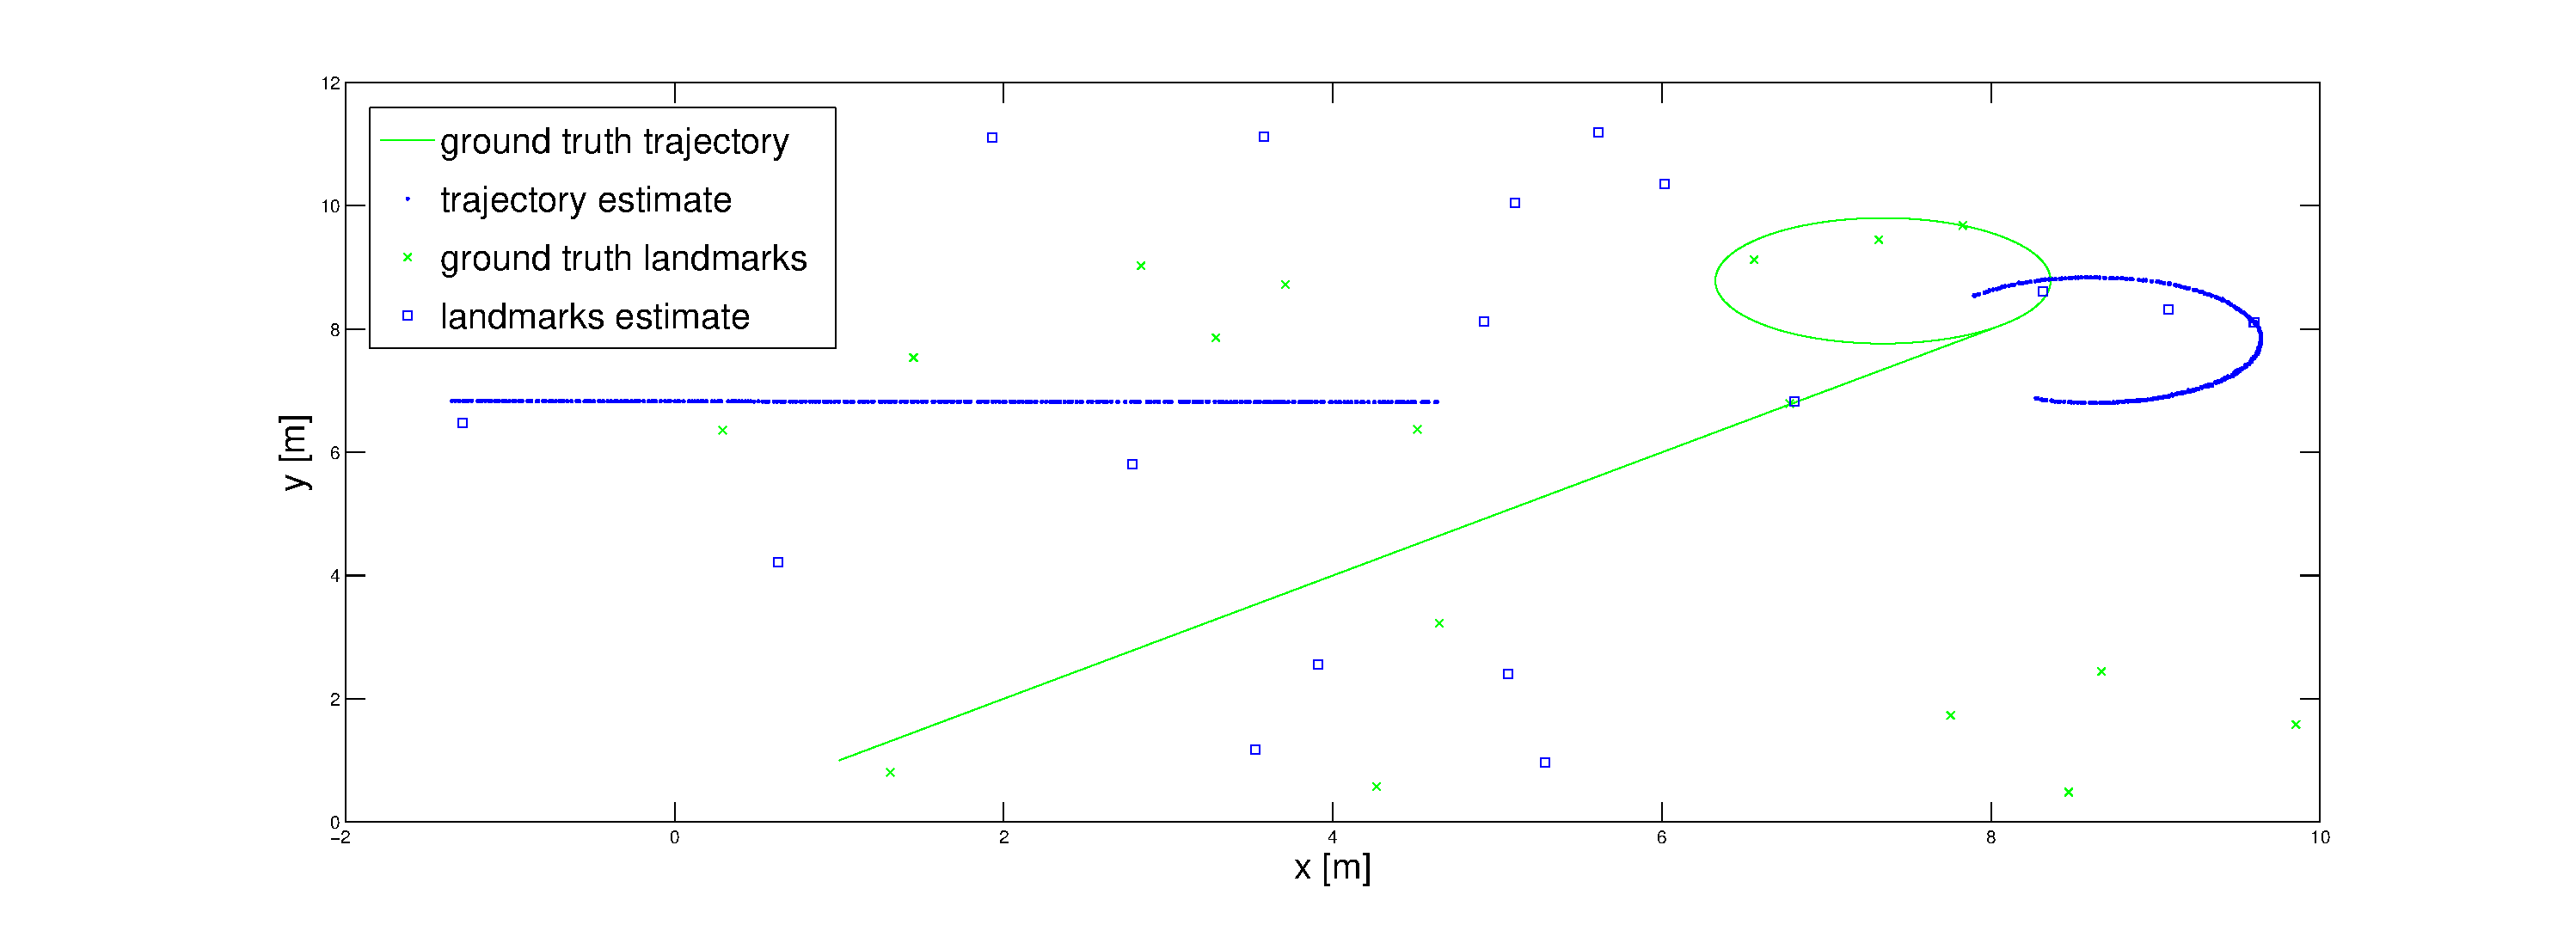
\includegraphics[width=\columnwidth]{fig/slam_calib_it3.eps}
\caption{Exemplary output of our calibration algorithm (best viewed in
color). The ground truth trajectory and landmark positions are shown in green
and their respective estimates in blue. While dealing with degenerate cases, our
method only selects batches of data that provide enough information to the
estimator. In this example, the observed shift in the estimate comes from the
absence of any prior information.}
\label{fig:calib_demo}
\end{figure}

The remainder of the paper is structured as follows. Section~\ref{sec:rel}
will give a brief overview over related approaches. Section~\ref{sec:model} is
dedicated to the mathematical grounding of our method.
Section~\ref{sec:exp} demonstrates the validity of our approach through
extensive experiments and evaluation. Section~\ref{sec:conc} will conclude the
paper.


\section{Related Work\label{sec:rel}}
The problem of sensor calibration has been a recurring one in the history of
robotics and computer vision. Thereby, it has been addressed using a
variety of sensor setups and algorithms. A calibration process may involve
recovering \emph{intrisic}, e.g. focal length for a camera, and \emph{extrinsic}
parameters, i.e. the rigid transformation between the sensor's coordinate system
and a reference coordinate system. For the former, one could devise a naive
approach where the parameters are accurately determined during the manufacturing
process. In the same vein, the transformation could be retrieved by means of
some measuring instrument. However, the disadvantages of such purely
engineered methods are manifolds. Apart from their impracticality, it can be
nearly impossible to reach a satisfying accuracy and thus hinder the proper use
of the sensor in a robotic system. Furthermore, external factors such as
temperature variations or mechanical shocks may seriously bias a factory
calibration. Therefore, much efforts have been dedicated over the years to
develop algorithms easing custom calibration on the field.

The use of a known calibration pattern such as a checkerboard coupled with
nonlinear regression has become the most popular method in computer vision
during the last decade. It has been deployed both for intrinsic camera
calibration~\cite{sturm99plane} and extrinsic calibration
between heterogeneous sensors~\cite{zhang04extrinsic}. While being relatively
efficient, this procedure still requires expert knowledge to reach a good level
of accuracy. It can also be quite inconvenient on a mobile platform requiring
frequent recalibration.

In the context of mobile robotics, several authors have included the calibration
problem in a state-space estimation framework,
either as filtering~\cite{martinelli06automatic}, or
smoothing~\cite{kuemmerle11simultaneous}.

List of papers to cite: \cite{davis11algorithm},
\cite{brookshire12extrinsic}, \cite{aster11parameter}, \cite{brookshire11automatic},
\cite{chan94lowrank}, \cite{finsterle11truncated}, \cite{golub96matrix},
\cite{hansen87truncated}, \cite{hong92rank}, \cite{jauffret07observability},
\cite{kitagawa01regularization}, \cite{levinson10unsupervised},
\cite{mackay05information}, \cite{maddern12lost},
\cite{sheehan12self}, \cite{sheehan10automatic},
\cite{gao10online}, \cite{hol10modeling}, \cite{kaess09covariance}


\section{Model\label{sec:model}}
\documentclass[12pt]{article}
\usepackage{amsmath, amsfonts, amssymb}
\DeclareMathOperator*{\argmax}{arg\,max}
\DeclareMathOperator*{\argmin}{arg\,min}
\DeclareMathOperator{\diag}{diag}
\DeclareMathOperator{\rank}{rank}
\title{Toyota PRIUS Calibration}
\author{J\'{e}r\^{o}me Maye}
\date{\today}
\begin{document}
  \maketitle
  \section{Model}\label{sec:model}
\end{document}


\section{Experiments\label{sec:exp}}
In order to evaluate and validate the approach proposed in this paper, we have
conducted experiments on simulated and real-world data. We shall first start
with the description of the experimental conditions and then demonstrate the
performance of our algorithm, along with some comparisons against existing
methods.

\subsection{Experimental Setup}

In our experiments, we consider the problem of a mobile robot moving on a plane.
Fig.~\ref{fig:exp_setup} depicts our experimental setup. The platform is
equipped with a range sensor delivering range and bearing angles measurements.
The calibration parameters of the range sensor consist in the transformation of
its coordinate system to the robot's coordinate system. The platform is further
endowed with wheel odometers outputting translational and rotational speeds.
While navigating on the plane, the robot observes a known number of landmarks
through its range sensor. Despite the apparent simplicity of the setup, our
algorithm is flexible enough to cope with more complex scenarios, e.g., multiple
heterogeneous sensors or 3D motion.

\begin{figure}[t]
\centering
\missingfigure[figwidth=\columnwidth]{Experimental setup.}
\caption{Experimental setup.}
\label{fig:exp_setup}
\end{figure}

More formally, we use the following motion and observation models

\begin{equation}\label{eqn:exp_model}
  \begin{aligned}
  \underbrace {
  \begin{pmatrix}
  x_k\\
  y_k\\
  \theta_k
  \end{pmatrix}}_{\mathbf{x}_k}&=
  \underbrace{
  \begin{pmatrix}
  x_{k-1}\\
  y_{k-1}\\
  \theta_{k-1}
  \end{pmatrix} + T
  \begin{pmatrix}
  \cos\theta_{k-1}&0\\
  \sin\theta_{k-1}&0\\
  0&1
  \end{pmatrix}
  \left(\begin{pmatrix}
  v_k\\
  w_k
  \end{pmatrix}
  + \mathbf{w}_k\right)
  }_{\mathbf{h}(\mathbf{x}_{k-1}, \mathbf{u}_k, \mathbf{w}_k)}\\
  a &= x_i - x_k - \delta_x\cos\theta_k + \delta_y\sin\theta_k\\
  b &= y_i - y_k - \delta_x\sin\theta_k - \delta_y\cos\theta_k\\
  \underbrace {
  \begin{pmatrix}
  r_k^i\\
  \phi_k^i
  \end{pmatrix} }_{\mathbf{z}_{k_i}}&=
  \underbrace {
  \begin{pmatrix}
  \sqrt{a^2 + b^2}\\
  \atan2(b, a) - \theta_k - \psi
  \end{pmatrix}
  + \mathbf{n}_k}_{\mathbf{g}(\mathbf{x}_{k}, \boldsymbol{\ell}_i,
    \boldsymbol{\Theta}, \mathbf{n}_k)},
  \end{aligned}
\end{equation}

\noindent where $\mathbf{x}_k=[x_k\;y_k\;\theta_k]^T$ denotes the robot pose at
timestep $k$, $T$ the sampling period, $\mathbf{u}_k=[v_k\;w_k]^T$ the measured
translational and rotational speeds, $\mathbf{z}_{k_i}=[r_k^i\;\phi_k^i]^T$ the
range and bearing observation of landmark $i$ with pose
$\boldsymbol{\ell}_i=[x_i\;y_i]^T$, $\mathbf{w}_k\sim\mathcal{N}(\mathbf{0},
\mathbf{Q}_k)$ with $\mathbf{Q}_k=\diag(\sigma^2_v,\sigma^2_w)$,
$\mathbf{n}_k\sim\mathcal{N}(\mathbf{0}, \mathbf{R}_k)$ with
$\mathbf{R}_k=\diag(\sigma^2_r,\sigma^2_\phi)$, and
$\mathbf{\Theta}=[\delta_x\;\delta_y\;\phi]^T$ the range sensor's calibration
parameters.

\subsection{Simulated Data}

In our simulation, we can generate various paths for the robot, along with
corresponding sensor measurements, and thus analyze the convergence of multiple
algorithms, especially in degenerate cases. We have created an environment
with $N=17$ landmarks uniformly distributed on a $10m\times 10m$ grid. We have
set the noise parameters empirically to $\sigma^2_v=4.4\times 10^{-3}$,
$\sigma^2_w=8.2\times 10^{-2}$, $\sigma^2_r=9.0036\times 10^{-4}$, and
$\sigma^2_\phi=6.7143\times 10^{-4}$. The calibration parameters are set to
$\delta_x=0.219$ [m], $\delta_y=0.1$ [m], and $\psi=\pi/4$ [rad].

In a first experiment, we have driven the robot along a straight path a $100$
times, maintaining identical initial conditions over the different runs, and
monitored the convergence of the calibration parameters.
Fig.~\ref{fig:straight_comp} shows the performance of different algorithms,
namely an Extended Kalman Filter (EKF) similar to~\cite{martinelli06automatic},
a standard batch non-linear least squares method without
regularization~\cite{kuemmerle11simultaneous}, and our TQR-MI approach.

\todo{more text to come discussing the results}

\begin{figure}[t]
\centering
\missingfigure[figwidth=\columnwidth]{A comparison of different algorithms.}
\caption{A comparison of different algorithms on a straight path.}
\label{fig:straight_comp}
\end{figure}

In a second step, we have run similar experiments as above, but with a loop
after the straight path. Fig.~\ref{fig:loop_comp} displays a comparison of the
different methods.

\todo{more text to come discussing the results}

\begin{figure}[t]
\centering
\missingfigure[figwidth=\columnwidth]{A comparison of different algorithms.}
\caption{A comparison of different algorithms on a well-behaved path.}
\label{fig:loop_comp}
\end{figure}

The last simulated experiment aims at analyzing the singular values, or the
diagonal elements of the $\mathbf{R}$ matrix, of the FIM.
Fig.~\ref{fig:sing_values} shows...
\todo{more text to come discussing the results}

\begin{figure}[t]
\centering
\missingfigure[figwidth=\columnwidth]{Singular values of the FIM.}
\caption{Singular values.}
\label{fig:sing_values}
\end{figure}

\subsection{Real-world Data}

In order to validate our method on real-world data, we have used the ``Lost in
the Woods Dataset'' provided with the courtesy of Tim Barfoot. This dataset
contains approximately $20$ minutes of a robot driving amongst a forest of
tubes which serve as landmarks. The ground truth comes from a motion capture
system that tracks robot motion and tube locations. Apart from the calibration
parameters, which are set to $\mathbf{\Theta}=[\delta_x=0.219\;\delta_y=0\;
\phi=0]^T$, the others remain unchanged.


\section{Conclusion\label{sec:conc}}
In this paper, we have presented a novel approach to the automatic calibration
of mobile robot sensors. We have included the calibration parameters in a SLAM
formulation and computed an MAP estimator using a Gauss-Newton algorithm. To
cope with unobservability, we have employed truncated QR decomposition as a
regularization method. For long-term and online operations, we have devised
a mutual information selection scheme that solely captures informative
measurements relevant to the calibration. Our algorithm has been thoroughly
tested and validated through extensive simulated and real-world experiments on
a 2D robot equipped with a laser range finder.

In the near future, we will consider the self calibration of multiple sensors
(cameras, 3D/2D LRF, GPS/INS system) mounted on an autonomous car and a C++
implementation. From a research point of view, we would like to further automate
the selection of the free parameters. Lastly, we want to detect stepwise changes
in the calibration parameters in order to trigger recalibration in case of
mechanical shocks.


\section*{Acknowledgment}
This work has partly been supported by the EC under ....

\bibliographystyle{sty/IEEEtran}
\bibliography{bib/bibliography}

\end{document}
